\documentclass[a4paper,11pt,openany,twoside,final,titlepage]{book}

\usepackage[latin1]{inputenc}
\usepackage[english]{babel}
\usepackage[T1]{fontenc}
\usepackage{graphicx}
\usepackage{amsmath} %Paquete para inculir formulas matematicas
\usepackage[right]{eurosym}
\usepackage{ifthen}
\usepackage{anysize}

\usepackage{textcomp}

\usepackage[hypertex]{hyperref}

\usepackage{syntonly}
%\syntaxonly % Comment this line to produce a pdf file

% Page Header and Foot
\usepackage{fancyhdr}
\setlength{\headheight}{15pt}

% Moves footnotes to the bottom of the page
%\usepackage[bottom]{footmisc}

% Makes possible to acces the name of the references and not only the numbers
\usepackage{nameref}

%\setlength{\parskip}{1ex plus 0.5ex minus 0.2ex}

% To be able to make acronyms
\usepackage[footnote]{acronym}
\acrodef{MiXiM}{Mixed Simulator}
\acrodef{WSN}{Wireless Sensor Networks}
\acrodef{LPL}{Low Power Localization}
\acrodef{OLP}{Optimized Listening Period}
\acrodef{MAC}{Media Access Control}
\acrodef{RSSI}{Received Signal Strength Indicator}
\acrodef{KO}{Knocked Out}
\acrodef{IEEE}{Institute of Electrical and Electronics Engineers}
\acrodef{WPAN}{Wireless Personal Area Networks}
\acrodef{LR-WPAN}{Low Rate WPAN}
\acrodef{PHY}{Physical Layer}
\acrodef{CSMA/CA}{Carrier Sense Multiple Access with Collision Avoidance}
\acrodef{GTS}{Guaranteed Time Slot}
\acrodef{ACK}{Acknowledgement}
\acrodef{RFD}{Reduced Function Device}
\acrodef{FFD}{Full Function Device}
\acrodef{ED}{Energy Detection}
\acrodef{LQI}{Link Quality Indication}
\acrodef{CCA}{Clear Channel Assessment}
\acrodef{O-QPSK}{Offset quadrature phase-shift keying}
\acrodef{Tx}{Transmission}
\acrodef{Rx}{Reception}
\acrodef{PDA}{Personal Data Assistant}
\acrodef{MP3}{Moving Picture Experts Group Audio Layer III}
\acrodef{MATLAB}{Matrix Laboratory}
\acrodef{CD}{Compact Disk}
\acrodef{NB}{Number of BackOffs}
\acrodef{BE}{BackOff Exponent}
\acrodef{CAF}{Channel Access Failure}
\acrodef{SIFS}{Short Inter Frame Spacing}
\acrodef{LIFS}{Long Inter Frame Spacing}
\acrodef{MHR}{MAC Header}
\acrodef{MFR}{MAC Footer}
\acrodef{FCS}{Frame Control Sequence}
\acrodef{CRC}{Cyclic Redundancy Code}
\acrodef{PAN}{Personal Area Networks}
\acrodef{uC}[$\mu$C]{MicroController}
\acrodef{AN}{Anchor Node}
\acrodef{MN}{Mobile Node}

\author{Jorge P\'erez Hidalgo}
\title{Cosas con Noditos}
\date{\today}

\marginsize{3cm}{2cm}{2cm}{2cm}

%\renewcommand{\baselinestretch}{1.5}

\begin{document}

\pagestyle{empty}

\begin{center}
  \begin{figure}[ht]
    \begin{center}
      
\includegraphics[scale=1]{logo_tud.eps}
    \end{center}
  \end{figure}
  \vspace{0.2cm}
  \Large{\textbf{FAKULT\"AT ELEKTROTECHNIK\\ UND INFORMATIONSTECHNIK}}\\
  \vspace{0.5cm}
  \Large{\textbf{LEHRSTUHL F\"UR TELEKOMMUNIKATION}}\\
  \vspace{4cm}
  \Huge{\textbf{Simulative study of a high configurable protocol for localization in sensor networks}}\\
  \vspace{3cm}
  \Large{\textbf{FINAL PROJECT}}\\
  \vspace{0.5cm}
  \large{\textbf{INGENIER\'IA DE TELECOMUNICACI\'ON}}\\
\end{center}

\vspace{4cm}
\centerline{\llap{\textsc{autor:}} \rlap{ Jorge P\'erez Hidalgo}}
\vspace{0.2cm}
\centerline{\llap{\textsc{Betreuer:}} \rlap{ Dipl.~Ing.~Jorge Juan Robles}}



% First pages before the content of the document
\frontmatter

\pagestyle{plain}

\chapter*{\begin{it}Acknowledgements\end{it}}
\begin{quotation}
To my bichito :)
\end{quotation}
\pagestyle{empty}
\cleardoublepage

\chapter*{\begin{it}Abstract\end{it}}
\begin{quotation}
Nobody can hesitate about the importance of technology in our lives. This technology helps us in many applications, 
some of them can be done without any environment knowledge, but many others cannot. Whenever the situation is an important
issue (obtaining some information of the place I am, how to reach a determinate room, how full my fridge is \ldots), a way
to detect our position is needed.

Many systems try to fulfill this task, but not all are suitable in all scenarios. 802.15.4 beacon-less \ac{WSN} are chosen as an easy, cheap, 
low consumption and portable structure to achieve this aim. There are many ways to obtain an specific position. In this 
work, \ac{RSSI} from received packets will be used. The more \ac{RSSI} values and the more strength, the more exactitude obtained, but also 
the more energy is needed. Energy is hence, an important parameter in this process, and to try to reduce its consumption, 
this work purposes a high configurable protocol which permits to adjust this energy-exactitude compromise as needed, depending
on the context. In this work a framework for the OmNet++ network simulator is developed and different situations are 
analyzed to show the improvement of this protocol compared with the existing ones.
\end{quotation}
\pagestyle{empty}
\cleardoublepage

% Prints the content index
\tableofcontents

% Prints the figure index

% Pages with the content of the document
\mainmatter

\pagestyle{fancy}
\renewcommand{\sectionmark}[1]{
\lhead{\thesection.\ #1}}
\rhead{\thepage}
\cfoot{}


\chapter{Introduction}
\label{chap:introduction}

We are inside the information era, it is even said that information means money. It is clear then, that acceding to this information
everywhere and every time is an important issue. Thanks to telecommunication advances and the need of this information, it is
possible now to be permanently connected. Technology has also made devices smaller, cheaper and more powerful
every day (\ac{PDA}, Mobile Telephones, \ac{MP3} Players \ldots). All this together has created the \ac{WPAN} concept, a way 
all this devices can be interconnected, so they can complement each other to obtain applications beyond our imagination. The 
problem in this idyllic world is an old problem, energy. All this devices are supplied with batteries, what means that their 
lives are not so long until we must plug them in to continue working with them. This is the reason why it is necessary to build them
a way they reduce its energy consumption.

With the objective of creating an standard for this \ac{WPAN}, the \ac{IEEE}, created the 802.15 group, which created different 
kind of networks attending to the data rate. Among this kind of networks it is found the 802.15.4, designed for low data rates but 
also for low consumption. This standard is the one this work is based on.

\section{Why \ac{WSN}?}

As a cabled technology would be unpractical for a topology where free of movement is a must, it is clear the need of a 
wireless technology, but why did we choose 802.15.4 \ac{WSN} and not other alternatives?

One possible alternative would have been Wi-Fi. This technology is based in \ac{IEEE} 802.11 standard, and with bit rates up to
54 Mbps and much bigger ranges, would be a good alternative, but its energy consumption is much bigger than for 802.15.4 \ac{WSN}.

In the same group as \ac{WSN}, it can be found the Bluetooth (\ac{IEEE} 802.15.1), this standard has still bigger bit rates as 
802.15.4, but its energy consumption is still too big, as it is not thought for this kind of applications. Also Bluetooth scalability
is not as good as for 802.15.4.

This reasons together with the low prices of 802.15.4 compared with the other alternatives, made this work use the \ac{IEEE} 802.15.4 
standard as the standard for building a High Configurable Protocol for localization. The idea is that using this protocol we should
get a little node working with a couple of AA batteries for many months or even some years.

\section{Applications}

\ac{WSN} applications are wide and diverse, this application areas are just some examples:

\begin{itemize}
 \item \textbf{Medicine.} As the nodes size is every time smaller, some patients with problems which should be controlled all the time,
could find this networks really useful.
 \item \textbf{Security environments.} Places with toxic substances, where there cannot be humans, and where some parameters should be measured,
or delicate places that need the presence of sensors 24/7 to check that there was no intruders. This could be done also by \ac{WSN}.
 \item \textbf{Environmental sensors.} Vast areas like forests, sees, coasts \ldots that need to be controlled in some parameters like
humidity, temperature, fire, seismic activity \ldots which are impossible to be controlled by humans, are good controlled with sensors
and at the same time they minimize the environmental impact.
 \item \textbf{Industrial sensors.} The size of the sensors makes possible to access every corner of the industrial process, and it is also
possible to control much more parameters.
 \item \textbf{Indoor positioning.} Sensor make possible to be guided inside a building we don't know, or even to people with some handicaps.
They are also good to locate determinate objects in a building.
 \item \textbf{Home automation.} Every element in our house could have a sensor inside, they could communicate among them and even notify us
about some alerts or needs from the house, they could even check how we feel to prepare the house in a specific way.
\end{itemize}

Table \ref{tab:wsn_applications} was made from all this applications and many more. This table reflects a summary, and also divides and groups
the applications according to the priority in energy, accuracy and emergency, and also if the involved device needs to obtain some information
from the network. Priority in energy means that the other parameters do not matter too much, saving energy is the important task. 
The same happens with accuracy and with emergency, where the rest does not matter, the exact position or speed are needed.

\begin{table}[h]\footnotesize
\begin{center}
 \begin{tabular}{l||cccc}
  \noalign{\vspace*{0.5cm}}
  & \textbf{Consume} & \textbf{Accuracy} & \textbf{Emergency} & \textbf{Do I need} \\
  & \textbf{Priority} & \textbf{Priority} & \textbf{Priority} & \textbf{some data?} \\
  \hline\hline
  \textbf{Guided System} & High & High & Very High & Yes \\
  \hline 
  \textbf{Routine inspection in mobile stations} & Very High & High & Low & No \\
  \hline
  \textbf{Objects localization with accuracy} & High & High & Low & No \\
  \hline
  \textbf{Get some data about my position} & High & High & Low & Yes \\
  \hline
  \textbf{Objects localization with emergency} & High & Low & High & No \\
  \hline
  \textbf{Big objects with battery localization} & Very High & Low & Low & No \\
  \hline
  \textbf{Routine inspection in fixed stations} & Very High & Very Low & Low & No \\
  \hline
  \textbf{Get position with low energy consumption} & Very High & Low & Low & Yes \\
  \hline
  \textbf{Emergency measurement in mobile stations} & Low & High & Very High & No \\
  \hline
  \textbf{Emergency measurement in fixed stations} & Low & Very Low & Very High & No \\
  \hline
  \textbf{Plugged in objects localization} & Very Low & Low & Low & No \\
  \hline
  \textbf{High accuracy localization at any price} & Very Low & Very High & Very Low & No \\
  \hline
  \end{tabular}
 \caption{Summed and grouped \ac{WSN} applications}
 \label{tab:wsn_applications}
\end{center}
\end{table}

Later on, this kind of applications will derive in 4 different types of nodes in our network.

\section{Challenges and Objectives}

The market demands low cost devices, able to build a network in a easy way, and capable to measure different parameters and react to them
or answer to determinate orders received from a central computer. As it was already said, the ability to move is an important issue, so is 
also localization, as the position is needed to be able to communicate with a device and to provide it the best information possible.

This standard nodes have not a big range, that is why all the end devices cannot connect directly with a central computer and a routers network 
is needed. This, makes necessary again a system to locate where the end devices are, as a routing path is needed to send the information.

All this, and the reasons stated before, are the reasons why the 802.15.4 standard was chosen to build up a High Configurable Protocol for 
localization with \ac{WSN}. But this is not just perfect, some challenges are still to solve:

\begin{itemize}
 \item \textbf{Energy.} End devices with movement capability are supplied with batteries, and unless we want to change the battery often,
a good protocol making the battery life longer is needed.
 \item \textbf{Scalability.} Networks can be small at the beginning, but they can grow rapidly and decrease again. A network that adapts 
dynamically to new conditions is also needed.
 \item \textbf{Adaptability.} Routers and above all end devices might be configured to save energy but an emergency could happen where they 
must communicate immediately and with reliability with a central computer, this is incompatible with energy saving. Hence, devices must be
adaptable to the circumstances.
 \item \textbf{Simplicity.} Devices must remain low cost and small, this means usually that hardware components have not a good performance
or big memory capacities. This is a strong constraint in the design, and that is why the protocol must remain simple.
\end{itemize}

The objective of this Final Project is hence, the design of a Protocol based in \ac{IEEE} 802.15.4 standard, able to deal with all the 
challenges before. But the objective is also the design of a robust and complete framework where future works could add more functionalities
or improve the existing ones without worrying about the communication or basic functionality.
As this is a design stage, simulation was chosen instead of testing directly on real devices. The simulation will be done with the Discrete 
Events Simulator OMNet++ 4 using the \ac{MiXiM} framework, and the results will be treated with \ac{MATLAB}, this tools will be commented later on.

\section{Document structure}

This Final Project tries to explain in a detailed way the design and test of a High Configurable Protocol for localization in \ac{WSN}. To 
fulfill this, the following document structure will be used:

\begin{itemize}
 \item \textbf{Chapter \ref{chap:introduction}: \nameref{chap:introduction}.} In the current chapter, different wireless solutions, applications
for \ac{WSN}, challenges and objectives were exposed.
 \item \textbf{Chapter \ref{chap:802154standard}: \nameref{chap:802154standard}.} In this chapter, aspects of the 802.15.4 standard needed
in the following chapters are presented. This chapter does not mean to be a detailed explanation of the standard.
 \item \textbf{Chapter \ref{chap:protocoldesign}: \nameref{chap:protocoldesign}.} This chapter comments briefly, existing solutions for the
presented challenges and proposes and explains a new protocol.
 \item \textbf{Chapter \ref{chap:protocolimplementation}: \nameref{chap:protocolimplementation}.} Here a detailed description of the protocol 
implementation is presented, preceded by an explanation of the tools, the functionalities they already implemented and how they were
improved.
 \item \textbf{Chapter \ref{chap:simulationandresults}: \nameref{chap:simulationandresults}.} Several scenarios are proposed, which after their
simulation, give some results that will be analyzed. The whole protocol will be simulated, but this chapter will also focus on one of the 
phases where deeper results will be obtained.
 \item \textbf{Chapter \ref{chap:conclusionsandfuture}: \nameref{chap:conclusionsandfuture}.} Conclusions from previous chapters will be 
exposed followed by possible new paths to follow after this work and improvements that could be done.
 \item \textbf{Appendix \ref{chap:installation}: \nameref{chap:installation}.} Detailed manual how to install and configure the source code in 
the \ac{CD}, to make easier a new person to continue working with it. Introduction to the version control system GIT, used in the development of 
this Final Project.
\end{itemize}


\chapter{802.15.4 Standard}
\label{chap:802154standard}

Work-group \ac{IEEE} 802.15 was formed to elaborate an standard for the \ac{WPAN}. Inside this work-group, the Task Group 4 
deals with the low binary rate ones, \ac{LR-WPAN}. First standard revision was approved in 2003 with the name of: ``Wireless 
Medium Access Control (MAC) and Physical Layer (PHY) Specifications for Low-Rate Wireless Personal Area Networks (LR-WPANs)'' 
\cite{IEEE802.15.4-2003}.

As it can be observed in the title, the standard defines only the Physical Layer and the \ac{MAC} Layer. Using this base, 
this work will build the Network, Transport and Application Layers to define all network behavior according to the proposed 
High Configurable Protocol.

\section{General Aspects of 802.15.4}

A \ac{LR-WPAN} is a low cost and easy communication network, it allows wireless connection for low binary rate and reduced 
energy consumption applications. This network must provide easy installation, low cost and low energy consumption, it should
also provide a good and reliable data transfer but staying flexible and simple. It cannot be forgotten that as a \ac{WPAN}, it
has a reduced range of work.

\ac{IEEE} 802.15.4 defines the protocol and device interconnection in a \ac{WPAN}, as the objective of this work is not to 
transcribe the standard, only the main characteristics will be presented, focusing later on, just on the important aspects
for this Final Project. To have a deeper view of the standard, refer to \cite{IEEE802.15.4-2003}.

\begin{itemize}
 \item \ac{PHY}: works in 868 MHz (1 ch), 915 MHz (10 ch) and 2450 MHz (16 ch) bands.
 \item Binary rates of 20 kb/s and 40 kb/s at low frequencies and 250 kb/s at 2450 MHz.
 \item Uses 16 bits logic addresses and 64 bits physic addresses.
 \item Possible to use \ac{GTS}.
 \item Channel access through \ac{CSMA/CA}.
 \item \ac{ACK} protocol to assure the communication reliability.
 \item Low consumption oriented.
 \item Provides an Energy Detection system.
 \item Provides a Link Quality Indicator mechanism.
\end{itemize}

Attending to the device functionality, they can be classified in 2 kinds:

\begin{itemize}
 \item \acl{FFD}, this devices have full capacity and functionality, they are the framework of the network. They can connect 
among them but also with other \ac{RFD}. They are usually plugged in, so energy here will not be a problem. They can provide 
information or act as routers to redirect this information. In every network, there should be one \ac{FFD} who works as \ac{WPAN}
Coordinator, depending on the topology (see Figure \ref{fig:WPAN_Network_Topologies}) all communications must go through the 
Coordinator or not. This Coordinator is usually connected to a central computer that deals with the complexer tasks in the system 
and distributes all the information to the rest of the devices. This devices will be refered as \ac{AN} during this work, as they
are the ones which would be fixed.
 \item \acl{RFD}, this devices have a reduce capacity and functionality as they are thought for easy tasks. This devices are
usually powered with battery and that is why the energy consumption reduction must be focused on them. They can connect only
\ac{FFD} and cannot handle high traffic loads. This devices will be refered as \ac{MN} during this work, as they are the ones with 
movement possibility.

\vspace*{1cm}

\begin{figure}[here]
 \begin{center}
  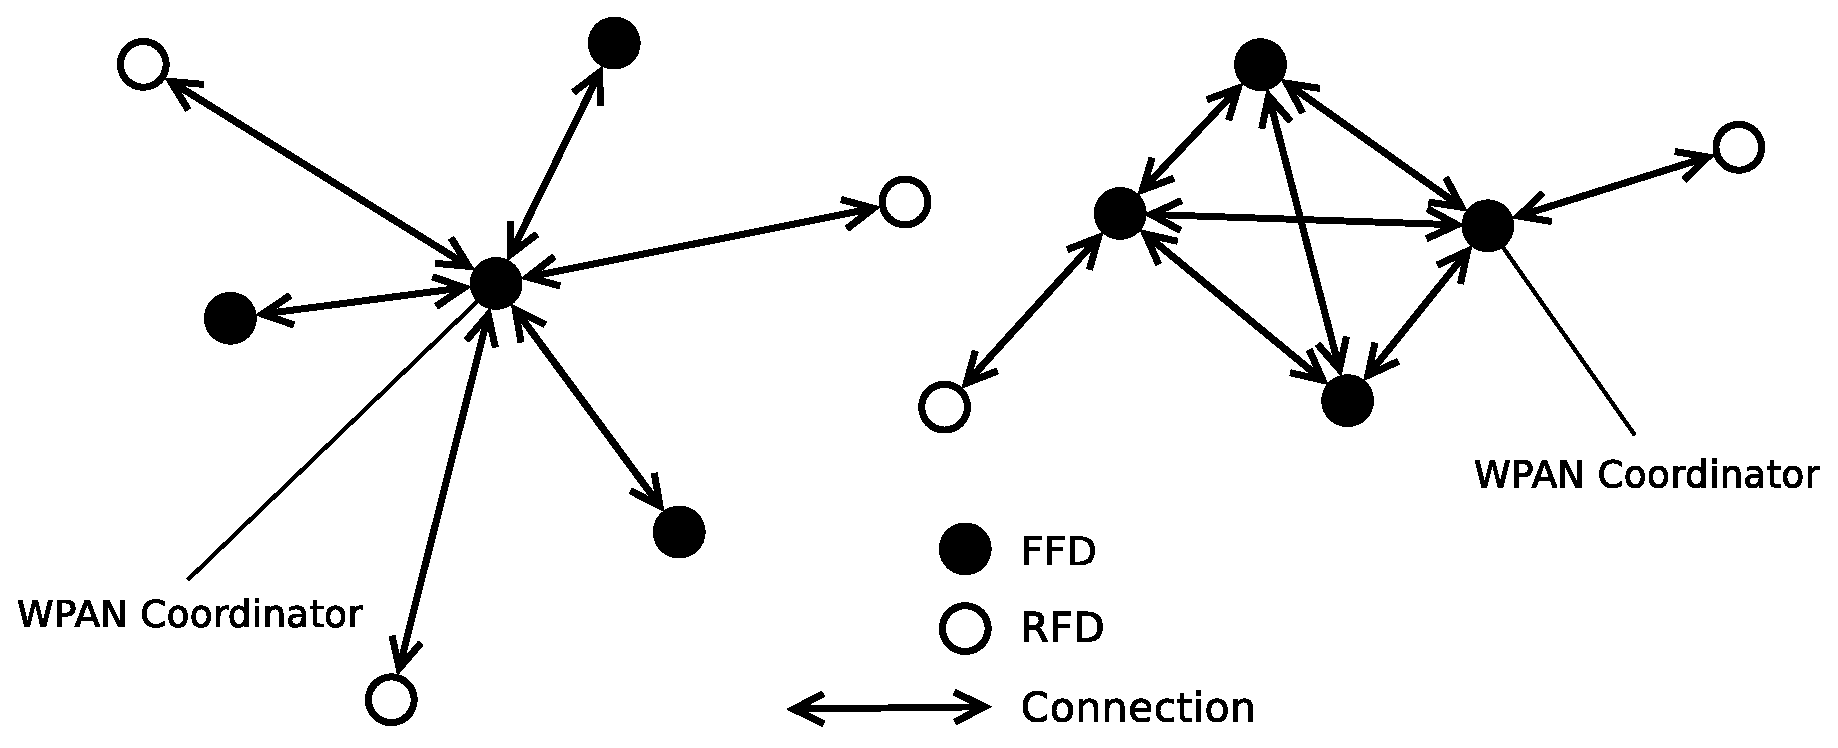
\includegraphics[width=0.9\textwidth]{WPAN_Network_Topologies.eps}
 \end{center}
 \caption{Star and peer-to-peer topology examples \cite{IEEE802.15.4-2003}}
 \label{fig:WPAN_Network_Topologies}
\end{figure}
\end{itemize}
This work will use the peer-to-peer topology as it is more flexible and scalable than the star topology. This topology is also
complexer, that is why a simpler case of peer-to-peer topology is selected, the tree topology. In this case all devices are
structured hierarchically and all of them have a father with whom they communicate, excepting the \ac{WPAN} Coordinator who is on the top of the network.

For this topology, a Network Layer (not provided in 802.15.4) is needed. For routing purposes only the short address (16 bits),
from the 2 kinds already commented, will be used. This is to make packets as short as possible (this happens only when the packet goes from and 
to a \ac{FFD}).

\section{Physic Layer}

Although for this work \ac{PHY} Layer has not as much importance as the \ac{MAC} Layer, there are some aspects that are important and 
that are good to know. This section will focus just on this aspects.

Some of the tasks developed by the \ac{PHY} Layer are:

\begin{itemize}
 \item \textbf{Switches on and off the radio transceiver.} Transceiver has 3 operation modes, \ac{Tx}, \ac{Rx} and sleeping, \ac{PHY}
layer must commute among this modes by \ac{MAC} layer petition. The standard defines that the change time between \ac{Rx} and 
\ac{Tx} and vice versa cannot be bigger as 12 symbols (\textit{aTurnaroundTime} = 12 symbols = 192 $\mu$s at 2.4 GHz).
 \item \textbf{Performs the \ac{ED} of the channel.} \ac{PHY} layer measures the power level of the channels to choose the best one
to transmit, this measurement lasts exactly 8 symbols.
 \item \textbf{Performs \ac{CCA} to check the channel.} This indicator is a part of \ac{CSMA/CA} algorithm as it will be seen later. The
\ac{CCA} is requested by the \ac{MAC} Layer and the \ac{PHY} Layer returns IDLE or BUSY depending on the channel situation. This \ac{CCA}
period lasts exactly like the \ac{ED}, 8 symbols (128 $\mu$s at 2.4 GHz).
 \item \textbf{Channel frequency selection.} As it was already commented, the 802.15.4 standard contemplates 3 different frequency 
ranges, although only the 2450 MHz will be used in this work. At this frequency, the standard stipulates 
the use of a \ac{O-QPSK} modulation with a symbol rate of 62,5 symbol/s. As this modulation makes 4 bit per symbol, we get 
a 250 bit/s bit rate. This frequency range, has 16 different channels with a 5 MHz separation between them, the number of 
this channels goes from 11 to 26.
 \item \textbf{Data transmission and reception.} According to the standard, the \ac{PHY} Layer must be able to transmit with a minimum
power of 1 mW and it must have a sensibility of at least -85 dBm \cite{IEEE802.15.4-2003}. Figure \ref{fig:PPDU} shows the physical level frame structure.

\vspace*{1cm}

\begin{figure}[here]
 \begin{center}
  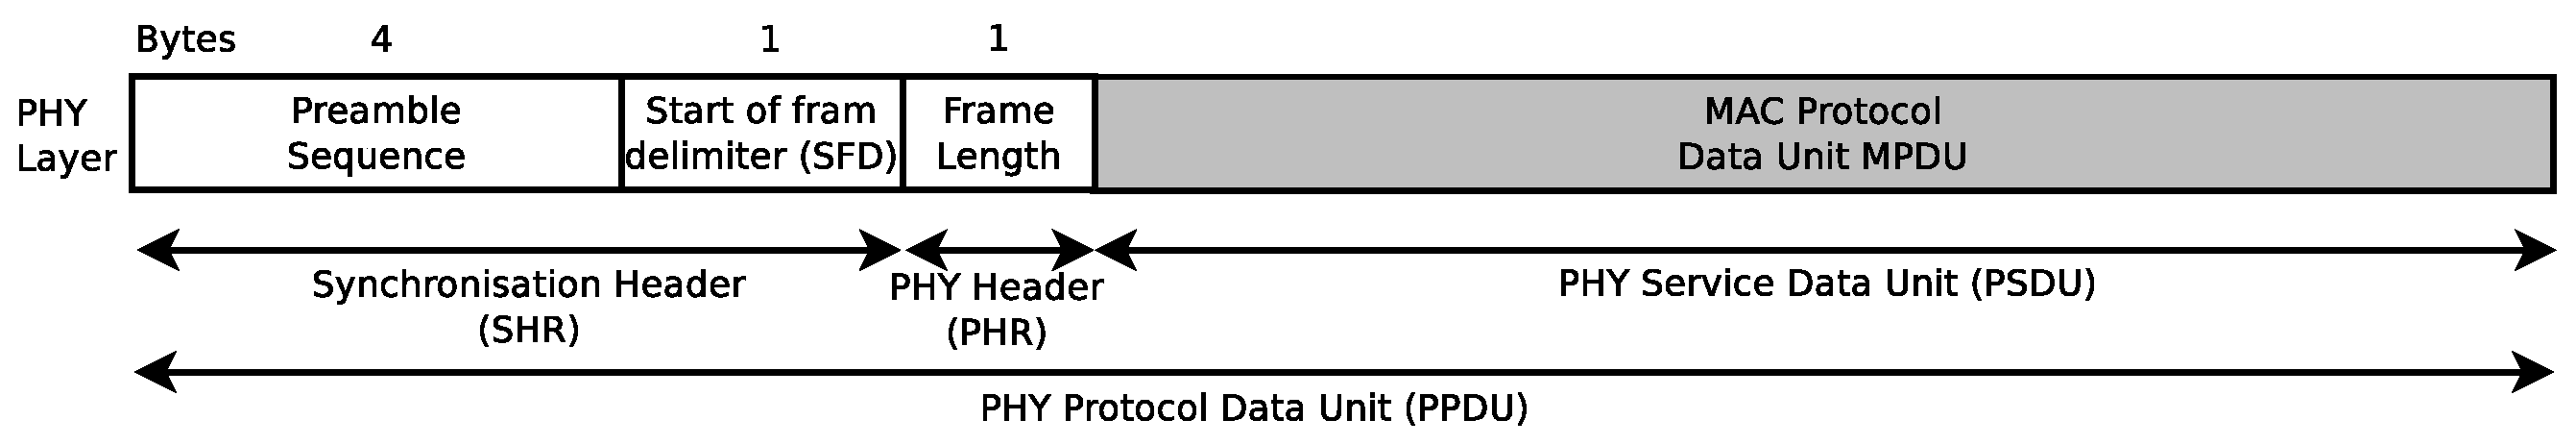
\includegraphics[width=0.9\textwidth]{PPDU.eps}
 \end{center}
 \caption{\ac{PHY} Layer frame \cite{IEEE802.15.4-2003}}
 \label{fig:PPDU}
\end{figure}
\end{itemize}

\section{\ac{MAC} Layer}

\ac{MAC} layer is the responsible for connecting the node with all the other nodes in a reachable distance. Although this layer has a reduced
primitive set (26 primitives), its really versatile and assures the minimum necessary to work. Some of the responsibilities of \ac{MAC}
layer are:

\begin{itemize}
 \item Assures a reliable link between two \ac{MAC} entities.
 \item Beacon generation if device is a router.
 \item Beacon synchronization.
 \item Nodes association and dissociation.
 \item Security mechanisms.
 \item Controls channel access through \ac{CSMA/CA}.
 \item Definition of \ac{GTS}.
 \item Frame validation.
 \item Duplicated received packets control.
 \item \ac{ACK} generation, this mechanism assures retransmission in \ac{MAC} layer, it is a transmission protection mechanism.
\end{itemize}

As happened for the \ac{PHY} layer, the \ac{MAC} layer has some constants and attributes to be configured, which will be used later in this work.
This parameters can be found from page 133 in \cite{IEEE802.15.4-2003}.

\subsection{Working Modes}

\ac{MAC} protocol supports 2 working modes, the coordinator is the one responsible to choose a mode when initializing the network:

\begin{itemize}
 \item \textbf{Beaconed mode.} In this mode, the coordinator generates a beacon and this is transmitted along the network thanks to the routers,
this beacon synchronizes all the devices in the network so they can sleep all the time and just wake up when they know the data will come. 
 \item \textbf{Non-Beaconed mode.} In this mode, the devices are not synchronized through beacons, that is why the routers and coordinator must
be awake all the time and the end devices are the only ones that can sleep. This is not a problem, as we assumed that \ac{FFD} would be plugged 
in and only \ac{RFD} would work with batteries. There is also the problem that end devices doesn't know when the data from the routers will come,
this will be solved through the proposed High Configurable Protocol.
\end{itemize}

Non-Beacon mode was selected for this work as it is more flexible for our purposes as Beaconed mode, this is too complex. But
this election has a problem, with beaconed mode all the sleep processes were automatically administrated by \ac{MAC} layer, now all the sleep 
and wake-up processes are still to be done by the Application Layer. From now on, all references will be assuming we are working with non-beaconed
mode.

\subsection{\ac{CSMA/CA} Algorithm}

When \ac{MAC} Layer receives a message to be sent, before sending it, asks the \ac{PHY} Layer to check if the channel is free and if so, it 
orders the \ac{PHY} Layer to transmit this message. This is all controlled by an algorithm, this algorithm is called \ac{CSMA/CA}, in this 
case as a non-beaconed mode is used, the \ac{CSMA/CA} algorithm corresponds to the non-slotted one, where the random time a device waits 
before transmitting is not synchronized with the beacons. A graphic approach to this algorithm is given in Figure \ref{fig:CSMACA}, where the
processes to be commented are signaled with number between brackets.

\begin{itemize}
 \item \textbf{(1)} - Restarts the parameters to its initial values. \ac{NB} is a counter of the number of times the process was done. \ac{BE}
is the exponent for the BackOff Random time calculation. At the beginning takes the minimum defined by the user (macMinBE), usually 3.
 \item \textbf{(2)} - In this step a random number between 0 and $2^{\ac{BE}}$ - 1 is generated and multiplied by the unit BackOff period, defined
by aUnitBackoffPeriod in the standard which default value is 20 symbols = 320 $\mu$s.
 \item \textbf{(3)} - After this waiting period where node is in IDLE mode, \ac{MAC} orders \ac{PHY} to sense the channel performing the \ac{CCA} 
(8 symbols = 128 $\mu$s) and if the channel is free, the \ac{MAC} proceed to transmit the packet and if not, the algorithm proceeds with the 
step (4).
 \item \textbf{(4)} - If the channel was busy, first \ac{NB} and \ac{BE} are raised in 1 unit, then if the new \ac{BE} is bigger than the maximum
(macMaxBE), usually 5, \ac{BE} is assigned this maximum value.
 \item \textbf{(5)} - Then maximum number of tries (macMaxCSMABackOffs) is checked, if the maximum is not reached, the process starts again from (2),
but if the maximum is reached, all process gets canceled and \ac{MAC} layer informs upper layers about the failure (\ac{CAF}).
\end{itemize}

\begin{figure}[!ht]
 \begin{center}
  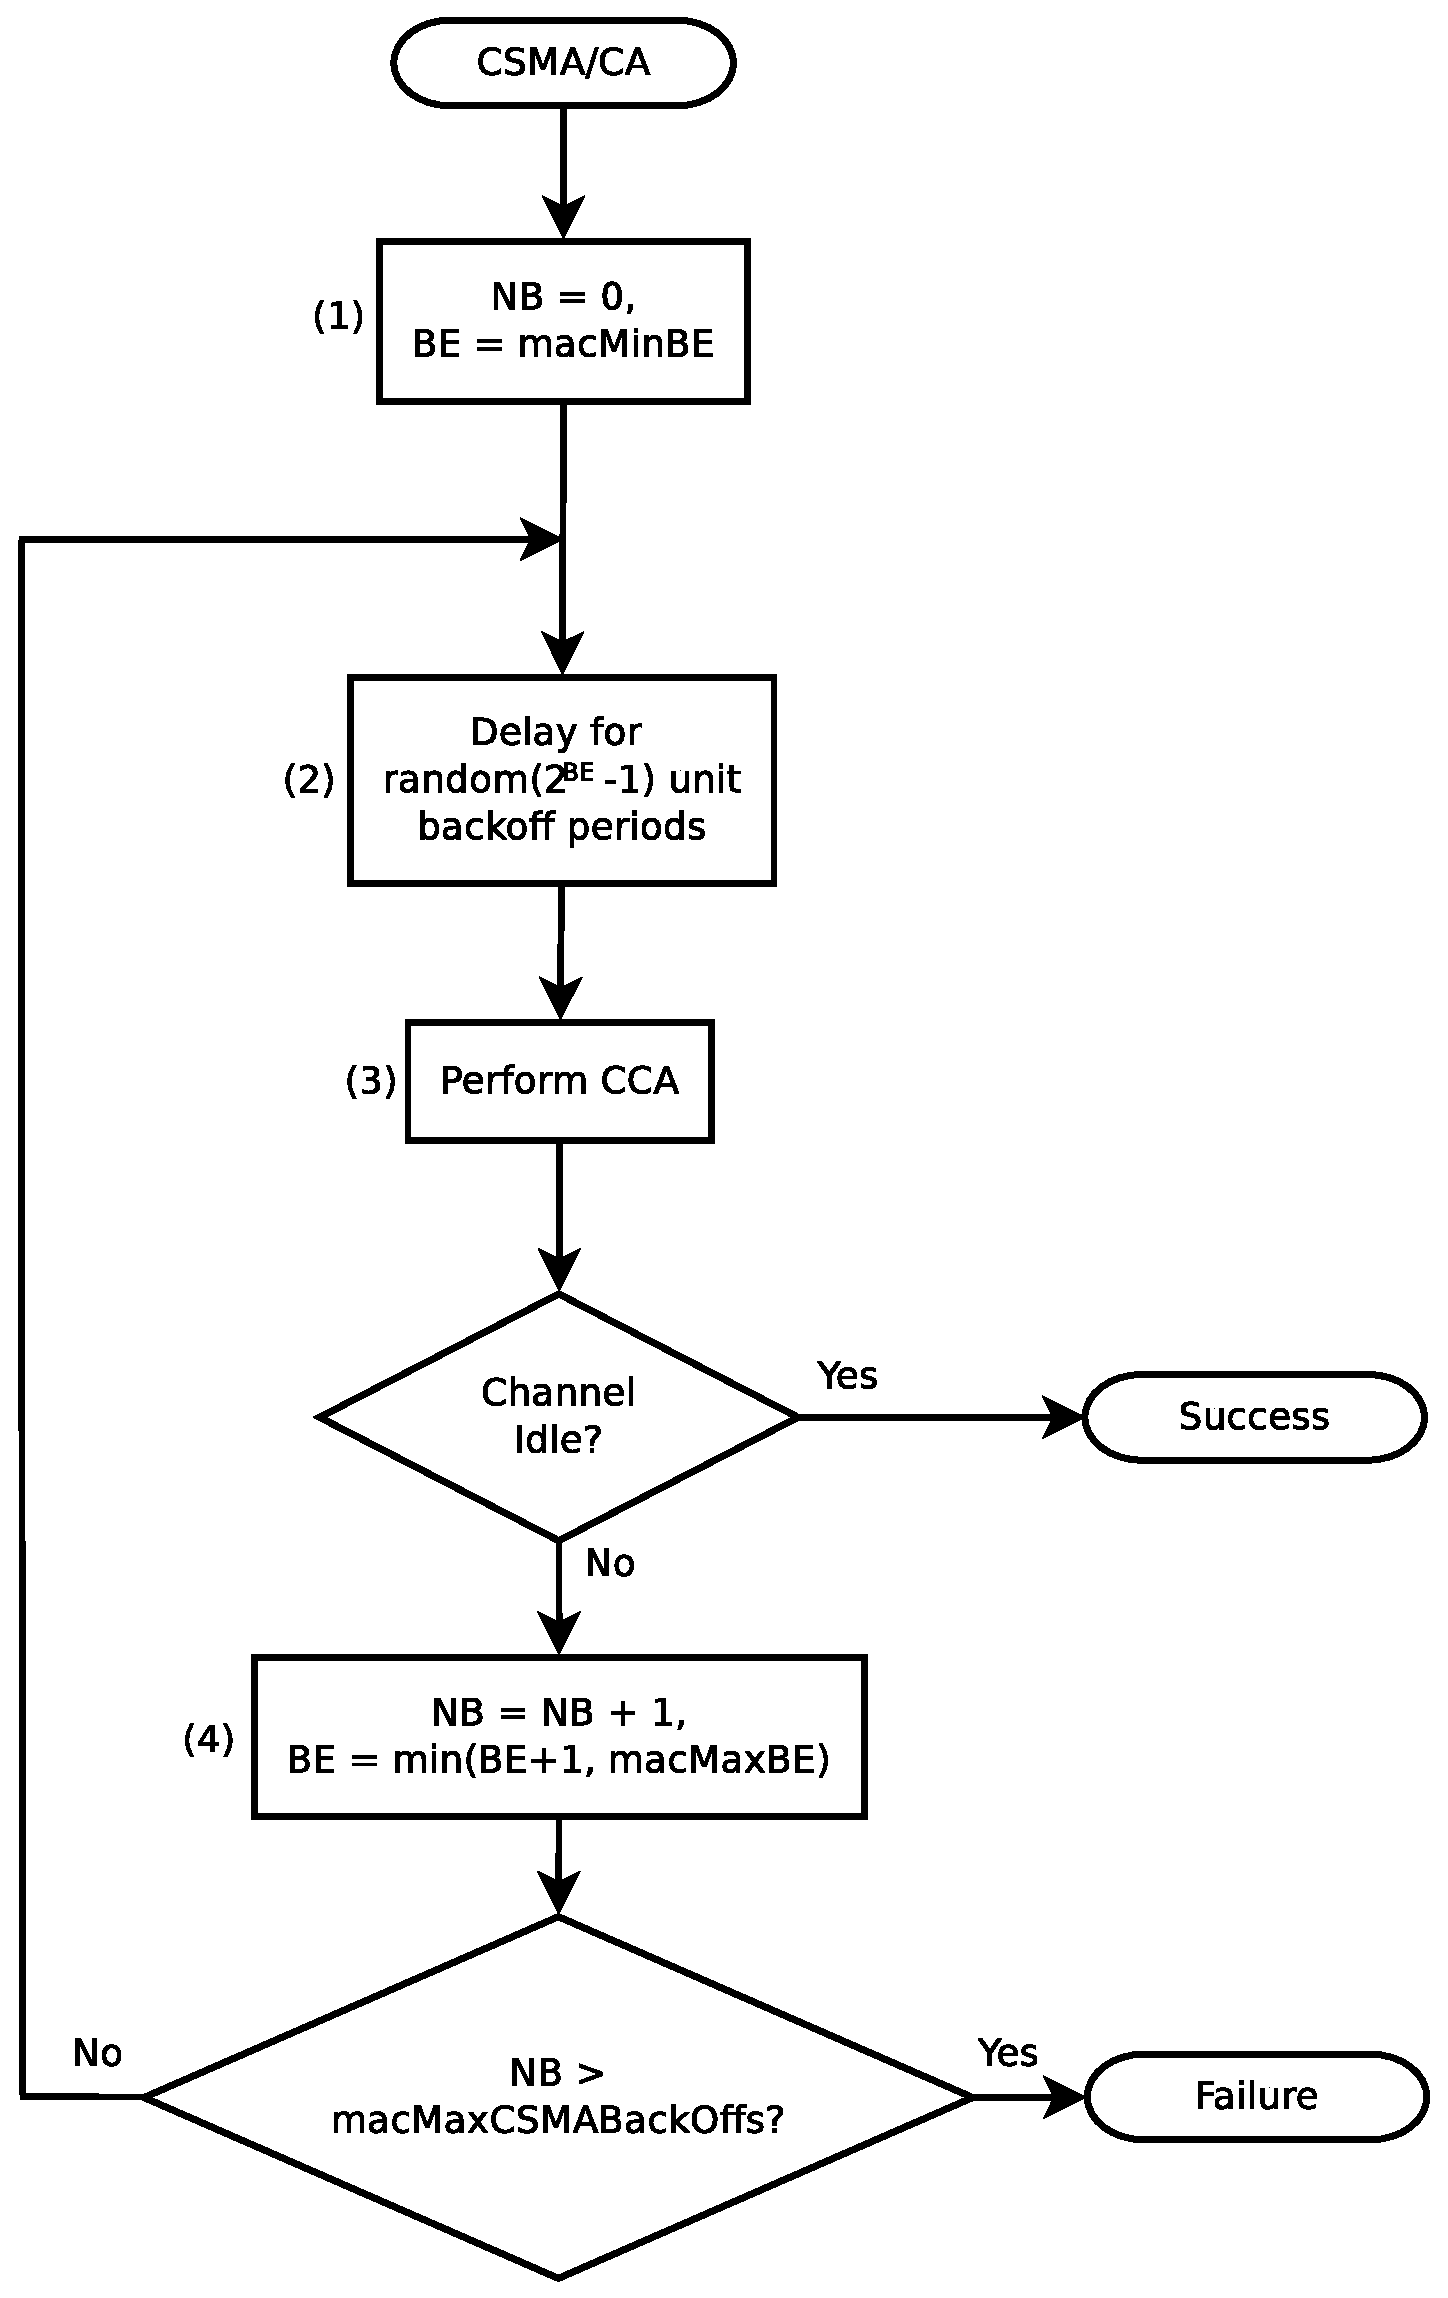
\includegraphics[width=0.5\textwidth]{CSMACA.eps}
 \end{center}
 \caption{Non-Slotted \ac{CSMA/CA} Algorithm}
 \label{fig:CSMACA}
\end{figure}

This algorithm helps to reduce the so called collisions. This collisions could occur when a node starts transmitting without looking the 
channel, and if another node next to it has already sent some packet, then a collision is produced.

But using \ac{CSMA/CA} algorithm does not make things perfect, it could also happen that two packets have a collision in the air. One 
reason could be that while one node is performing the \ac{CCA}, another node does the same, in this case, both of them will start transmitting 
producing a collision. The other reason is the well known Hidden Terminal Problem, to explain this phenomena, Figure \ref{fig:HiddenTerminalProblem}
will be used. Node A wants to communicate with node B, but node C is already transmitting something to node B, as we can see with the doted line,
A range does not cover node C, that is why when it performs the \ac{CCA}, does not get any signal from C. Then node A starts transmitting, and 
node B takes at the same time a message from A and C, having a collision.

\begin{figure}[!ht]
 \begin{center}
  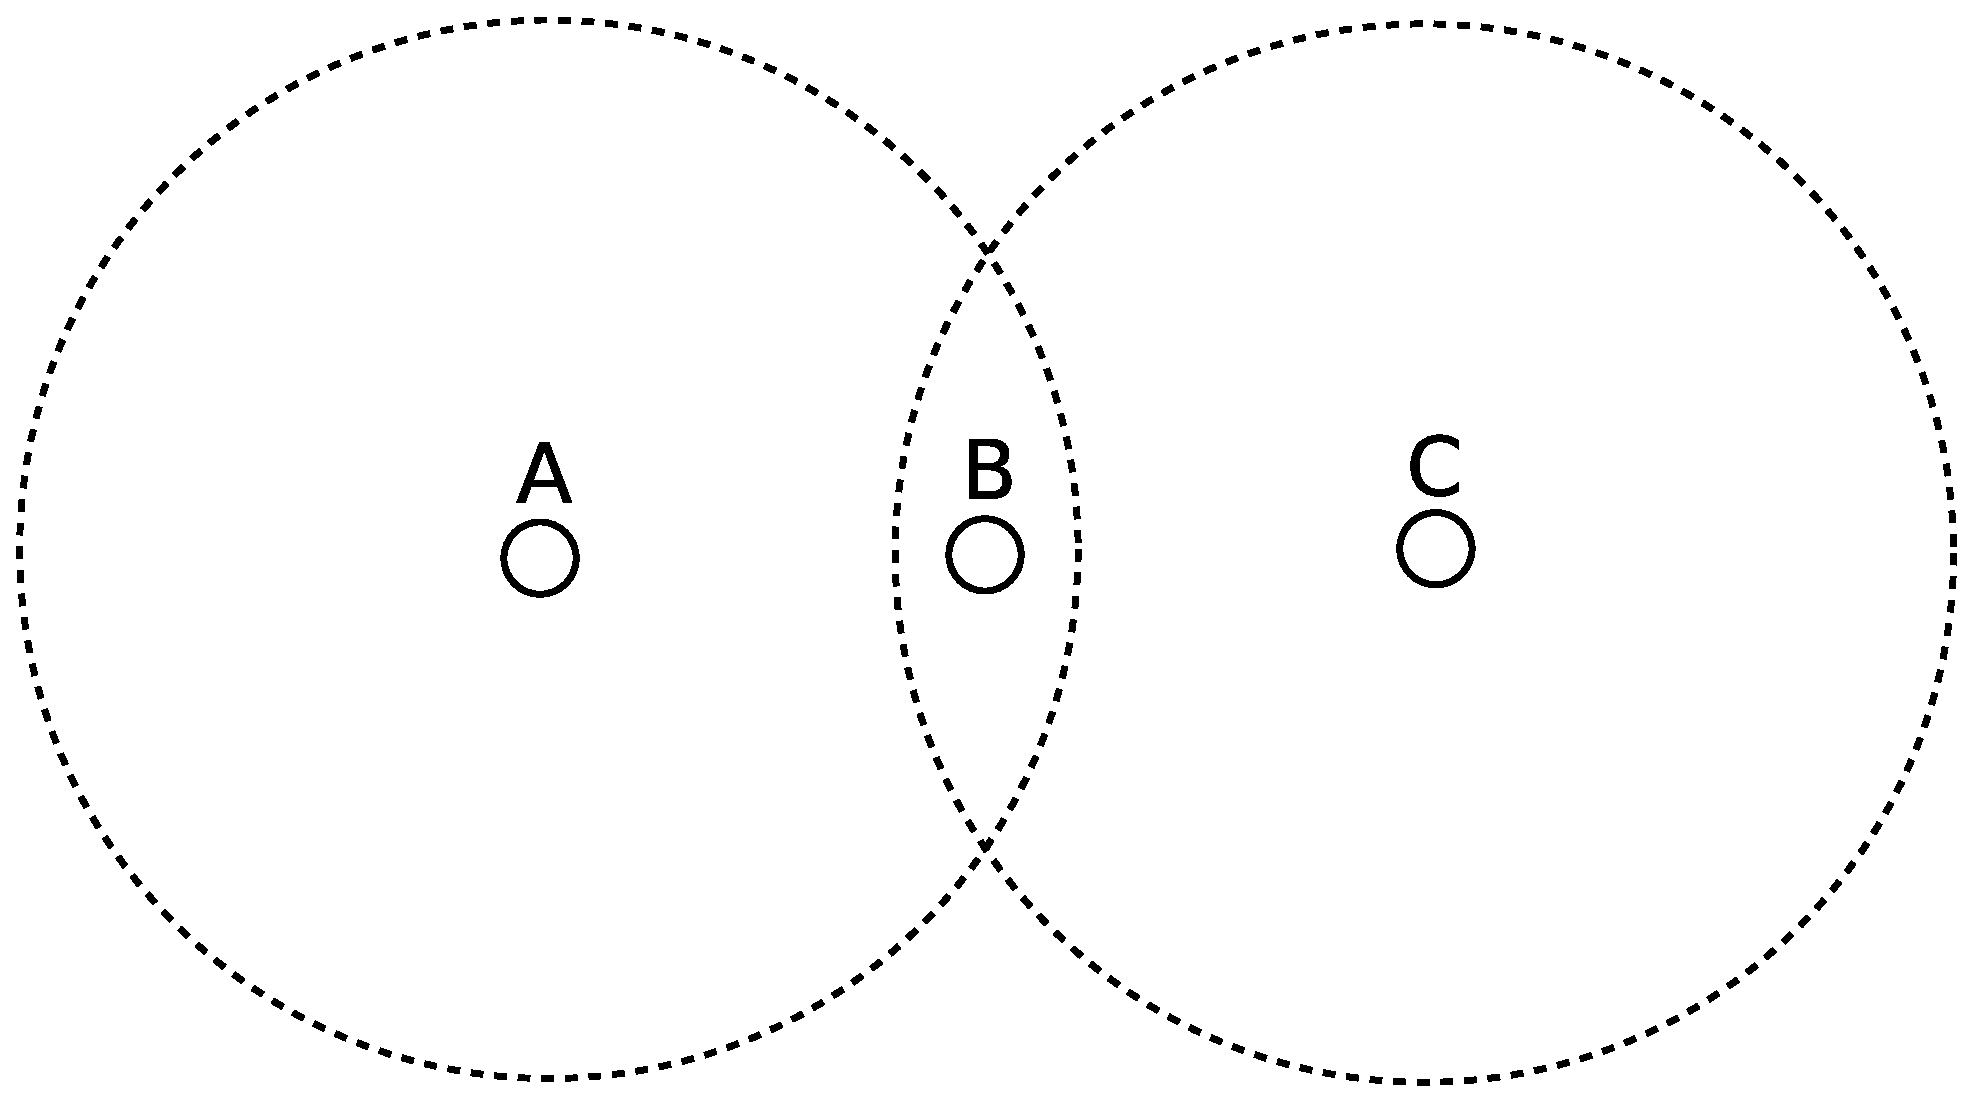
\includegraphics[width=0.3\textwidth]{HiddenTerminalProblem.eps}
 \end{center}
 \caption{Hidden Terminal Problem Scenario}
 \label{fig:HiddenTerminalProblem}
\end{figure}

\ac{CSMA/CA} algorithm makes also possible a situation where a node could transmit without collision but it detects a packet in the air and does
not transmit. To explain this case, Figure \ref{fig:ExposedNodeProblem} will be used. Suppose C is already transmitting something to D, 
then B wants to transmit something to A, and as B performs the \ac{CCA}, it detects the channel is busy with C to D packet. Then B waits another
BackOff random time and does not transmit, although it could, as its packet would have reached A and would have not disturbed D.

\begin{figure}[!ht]
 \begin{center}
  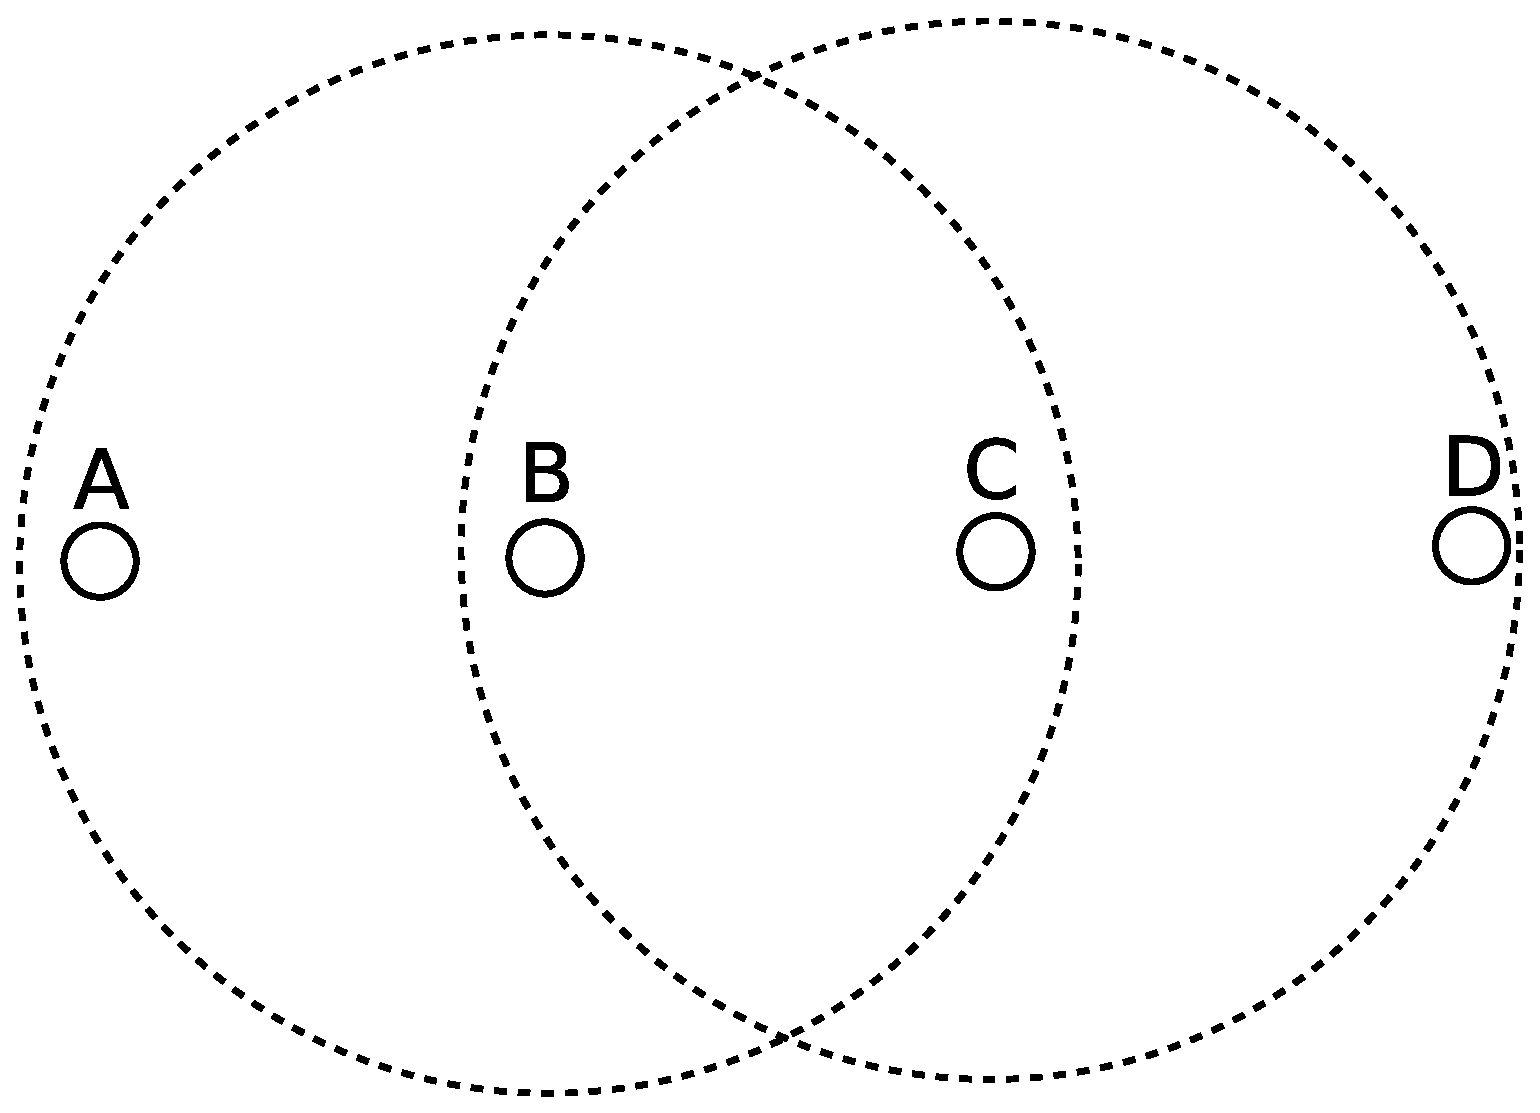
\includegraphics[width=0.3\textwidth]{ExposedNodeProblem.eps}
 \end{center}
 \caption{Exposed Node Problem Scenario}
 \label{fig:ExposedNodeProblem}
\end{figure}

Apart from the times already commented like \ac{CCA} or BackOff, there are other important times. \ac{SIFS} is the time to leave between two 
consecutive frames when the frame was short $(\le 18 bytes)$ and its value is 12 symbols = 192 $\mu$s. \ac{LIFS} is the same as \ac{SIFS} but
to use with long frames (40 symbols = 640 $\mu$s). Usually this two times are included in \ac{CSMA/CA} process, and they are important not to
collapse the system and loose data. Another important time is 
aTurnaroundTime, this time is 192 $\mu$s and corresponds to the time needed to switch between \ac{Rx} and \ac{Tx} modes and vice versa, it is
also the time to leave between the end of a packet reception and the start of the \ac{ACK} transmission.

\subsection{Frame Format}

\ac{MAC} packets use different frames depending if the network is beaconed or non-beaconed, as this work is using just the non-beaconed mode,
just the frames relative to this mode will be explained. Figure \ref{fig:MACFrame} contains the structure that will be explained now.

\begin{figure}[!ht]
 \begin{center}
  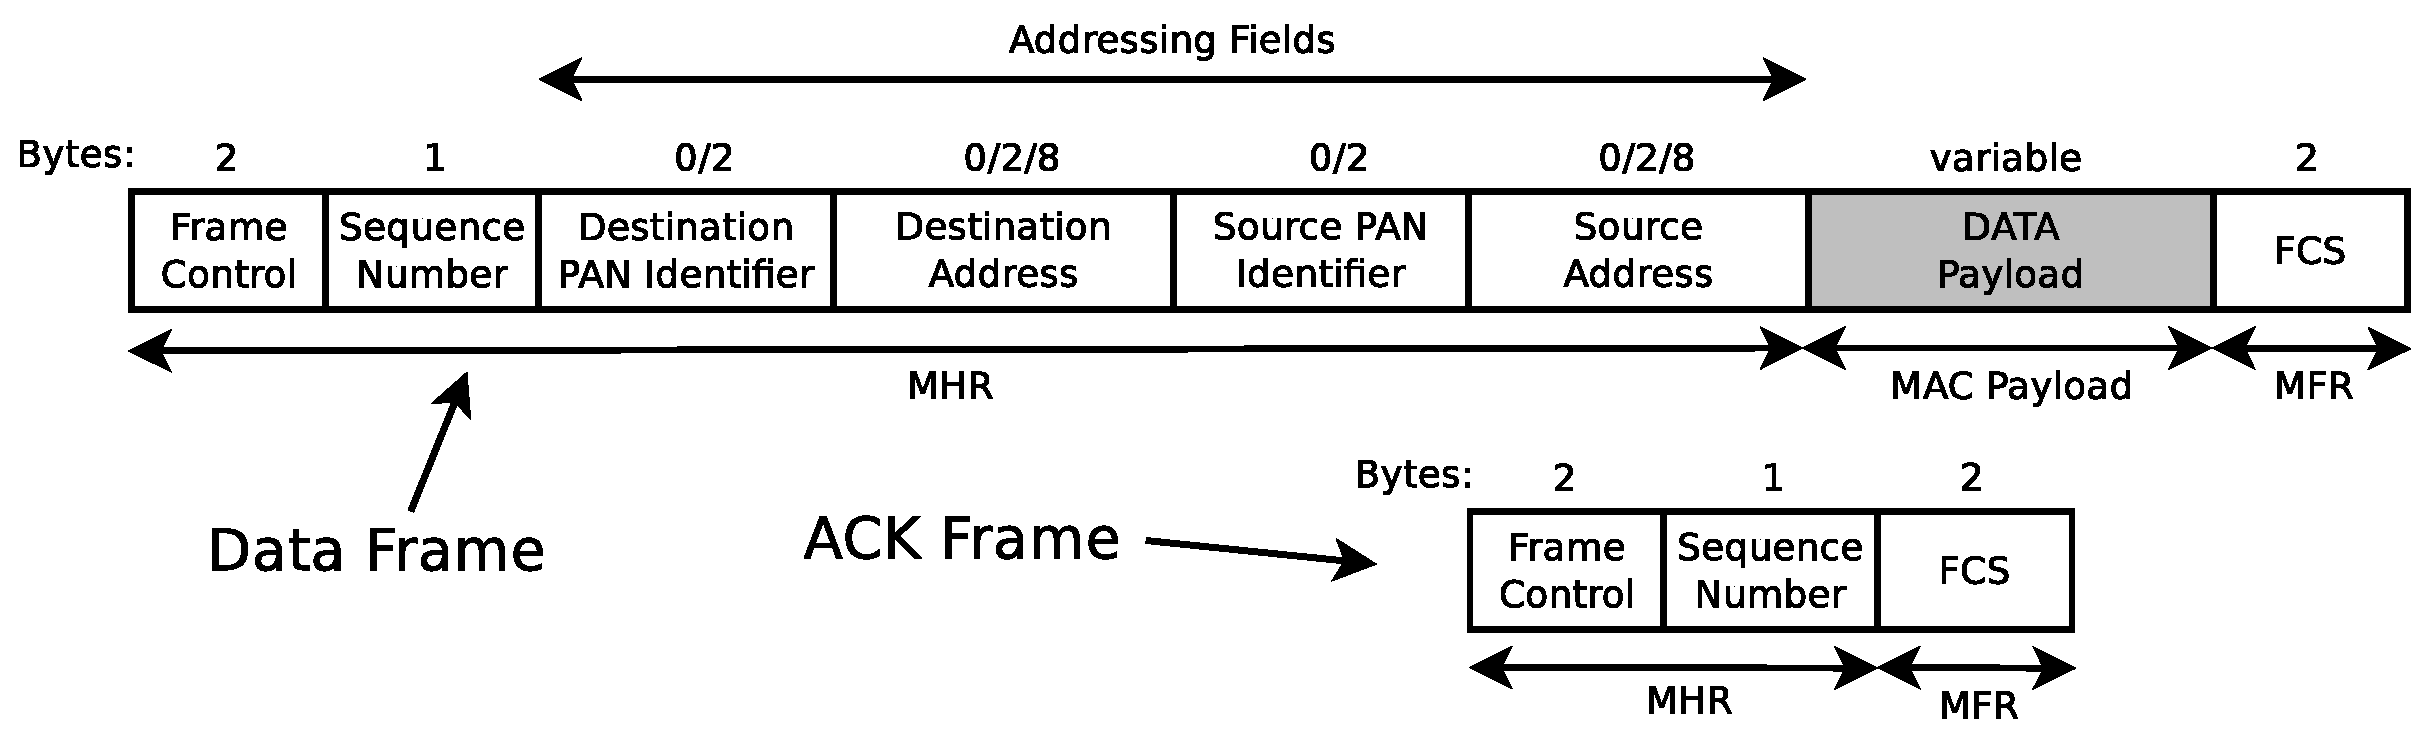
\includegraphics[width=0.7\textwidth]{MACFrame.eps}
 \end{center}
 \caption{Data and \ac{ACK} \ac{MAC} Frames}
 \label{fig:MACFrame}
\end{figure}

\begin{itemize}
 \item \textbf{Header (\ac{MHR}).} Formed by:
  \begin{itemize}
   \item Frame Control: 16 bits to define the frame type, security code, \ac{ACK} required, etc.
   \item Sequence Number: 8 bits to identify the frame.
   \item Destination \ac{PAN} Identifier: 16 bits to indicate the \ac{PAN} we are communicating with. 0xFFFF if any network is selected.
   \item Destination Address: 16 or 64 bits depending if it is a short or long address, end devices use always long address and routers short.
   \item Source PAN Identifier: 16 bits to indicate the \ac{PAN} that is communicating with us.
   \item Source Address: 16 or 64 bits depending if it is a short or long address, end devices use always long address and routers short.
  \end{itemize}
 \item \textbf{Payload.} Data from upper layer.
 \item \textbf{\ac{MFR}.} 16 bit sequence known as \ac{FCS}, this is a \ac{CRC}.
\end{itemize}

\subsection{Hardware}

Although this work is based in a simulation, all the needed physical parameters to simulate are obtained from the commercial hardware 
RCB230 V3.2 as is the one available in the department. This node has a AT86RF230 transceiver and a ATmega1281V \ac{uC}. According 
to \cite{LPLandOLP} the consumption values of this node can be seen in Table \ref{tab:NodeEnergyConsumption}, and transition times not defined
in 802.15.4 standard in Table \ref{tab:NodeTiming}.

\begin{table}[h]\footnotesize
\begin{center}
 \begin{tabular}{|l|c|}
  \noalign{\vspace*{0.5cm}}
  \hline
  & \textbf{Energy Consumption} \\
  \hline
  Transceiver in \ac{Rx} mode & 0.06496 mW/s \\
  \hline 
  Transceiver in \ac{Tx} mode & 0.06672 mW/s \\
  \hline
  Transceiver in IDLE mode & 0.04342 mW/s \\
  \hline
  Transceiver in Sleep mode & 0.0728 $\mu$W/s \\
  \hline
  \ac{uC} (Transceiver Sleeps) & 0.03042 mW/s \\
  \hline
  \end{tabular}
 \caption{Node RCB230 V3.2 Energy Consumption \cite{LPLandOLP}}
 \label{tab:NodeEnergyConsumption}
\end{center}
\end{table}

\begin{table}[h]\footnotesize
\begin{center}
 \begin{tabular}{|l|c|}
  \noalign{\vspace*{0.5cm}}
  \hline
  & \textbf{Transition timing} \\
  \hline
  Transition: Sleep -> \ac{Rx} & 1.88 ms \\
  \hline 
  Transition: \ac{Tx} -> Sleep & 0.94 ms \\
  \hline
  Transition: \ac{Rx} -> Sleep & 0.94 ms \\
  \hline
  \end{tabular}
 \caption{Transceiver AT86RF230 transition timing \cite{LPLandOLP}}
 \label{tab:NodeTiming}
\end{center}
\end{table}

\chapter{Protocol Design}
\label{chap:protocoldesign}

In the state of the art, there are different protocols constructed over \ac{IEEE} 802.15.4, like ZigBee, WirelessHART, 6LoWPAN \ldots \ some
are prepared for low consumption, others build different applications, but almost none of them are focused in localization. In the
department \ac{LPL} and \ac{OLP} \cite{LPLandOLP} protocols were proposed for this purpose. This protocols are based in \ac{IEEE} 802.15.4 and specifically 
designed for localization. In the next section a brief overview will be given, for a deeper view, please consult \cite{LPLandOLP}.

\section{\ac{LPL} and \ac{OLP}}

\ac{LPL} and \ac{OLP} \cite{LPLandOLP}, are two protocols designed for localization and based in \ac{RSSI} values. This values give an idea of 
the received signal strength in the device, and have the advantage that this information is already in all packets a device receives, there
is no need of special hardware or data to be prepared or obtained like in other methods (ultra wide band for example). But \ac{RSSI} values have 
a big problem for localization, its dispersion is very big, making the localization resolution (in some cases up to many meters 
\cite{fingerprint}) bad for some applications. 

This resolution problem, can be solved through some approaches. One kind is using localization techniques like ``fingerprint 
technique'' \cite{fingerprint} that improves the resolution. Another option is, taking more than 1 \ac{RSSI} value to obtain a more stable 
result. This technique has one big challenge, the more values are taken, the higher the energy consumption. Without a good approach, 
the \ac{MN} would need to listen to the channel most of the time waiting to receive packets from \ac{AN} to obtain \ac{RSSI} values, 
this way a lot of energy would be wasted just doing nothing, this is called idle listening. This 2 protocols propose 2 different 
approaches to solve this.

Another aspect in localization is who calculates the position, 3 different alternatives can be obtained.

\begin{itemize}
 \item \textbf{Centralized.} A central computer receives the \ac{RSSI} values from all \acp{AN} in the network and calculates the positions of 
the \acp{MN}. The advantage is that the computer can use complicate algorithms to obtain better results, but this method 
charges the network with a lot of traffic, specially if the \ac{MN} needs to know its position back after calculation.
 \item \textbf{Distributed-A.} The \ac{MN} sends the \ac{RSSI} values directly to the \ac{AN}, and this calculates directly the \ac{MN} position,
this does not charge the network so much like the centralized approach but the resolution is also not so good. It is important to note that 
each \ac{MN} has a ``selected \ac{AN}'', this \ac{AN} is the one in charge to calculate \ac{MN} position and the one the \ac{MN} communicates
with and through. This \ac{AN} is usually the one closest to the \ac{MN}.
 \item \textbf{Distributed-M.} In this mode, is the \ac{MN} who calculates directly its position from \ac{RSSI} values obtained from \acp{AN},
the problem is that \acp{MN} cannot use powerful localization algorithms. This solution is the one that almost does not charge the network.
\end{itemize}

The protocols \ac{LPL} and \ac{OLP} are going to use phases for different behaviors, and this phases will be repeated cyclically, that's why 
a good synchronization among all the nodes is necessary so all nodes can start the phases at the same time. Nodes will get 
the synchronization information from their parents (do not forget that a tree topology is used) using an active or a passive synchronization. 
To get a graphical explanation check Figure \ref{fig:synchronization}.

\begin{itemize}
 \item \textbf{Passive Synchronization.} The parent starts the process sending a packet R1 to \ac{MAC} to be transmitted, this packet is
created at the time-stamp Tx1, and includes this time, the time until the next phase start (TF) and info about this phase. Due to random time in 
\ac{CSMA/CA} process and other processing times, R1 is not transmitted immediately but in Tx2. When the packet is transmitted, \ac{MAC} informs
the application layer and this creates another packet (R2) including the new time-stamp Tx2. At the child, 2 packets will be received, R1 and 
R2 in times Rx1 and Rx2 respectively. Calculation of next phase start from the child point of view (TZ) is done like in (\ref{mat:pasivesync}).

\begin{equation}
  TZ = TF - (Rx2 - Rx1) - (Tx2 - Tx1)
  \label{mat:pasivesync}
\end{equation}

\begin{figure}[here]
 \begin{center}
  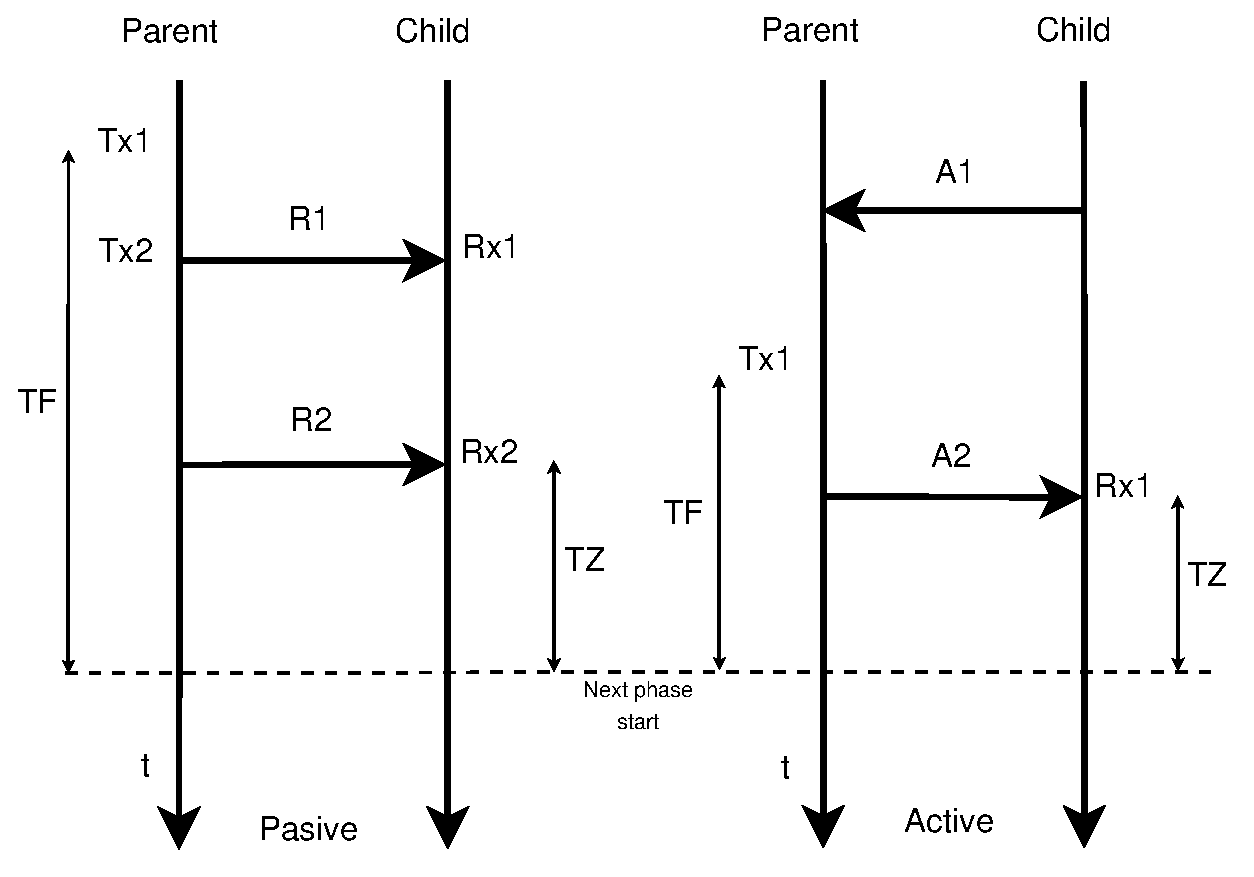
\includegraphics[width=0.6\textwidth]{synchronization.eps}
 \end{center}
 \caption{Passive and Active Synchronization \cite{LPLandOLP}}
 \label{fig:synchronization}
\end{figure}
 
 \item \textbf{Active Synchronization.} In the active synchronization, the child starts the process sending a synchronization request (A1),
then the parent answers with packet A2, this packet contains the time until the start of the next phase (TF). The child can calculate this time
with like in (\ref{mat:activesync}).

\begin{equation}
  TZ = TF - C
 \label{mat:activesync}
\end{equation}

The C parameter in (\ref{mat:activesync}), represents an estimation of all the processing times and random times from \ac{CSMA/CA}, that is why
this method is not so exact like the passive one, although it does not need 2 packets like it.
\end{itemize}

In the following subsections, both protocols \ac{LPL} and \ac {OLP} are going to be introduced.

\subsection{\acl{LPL}}

To reduce the idle listening, and thus the energy consumption, this protocol, proposes that instead of listening to the \acp{AN}, the
\acp{MN} are the ones who transmit and the \acp{AN} the ones who listen and transmit this information. This protocol is divided in 3 
phases which can be appreciated in Figure \ref{fig:LPL}.

\begin{figure}[h]
 \begin{center}
  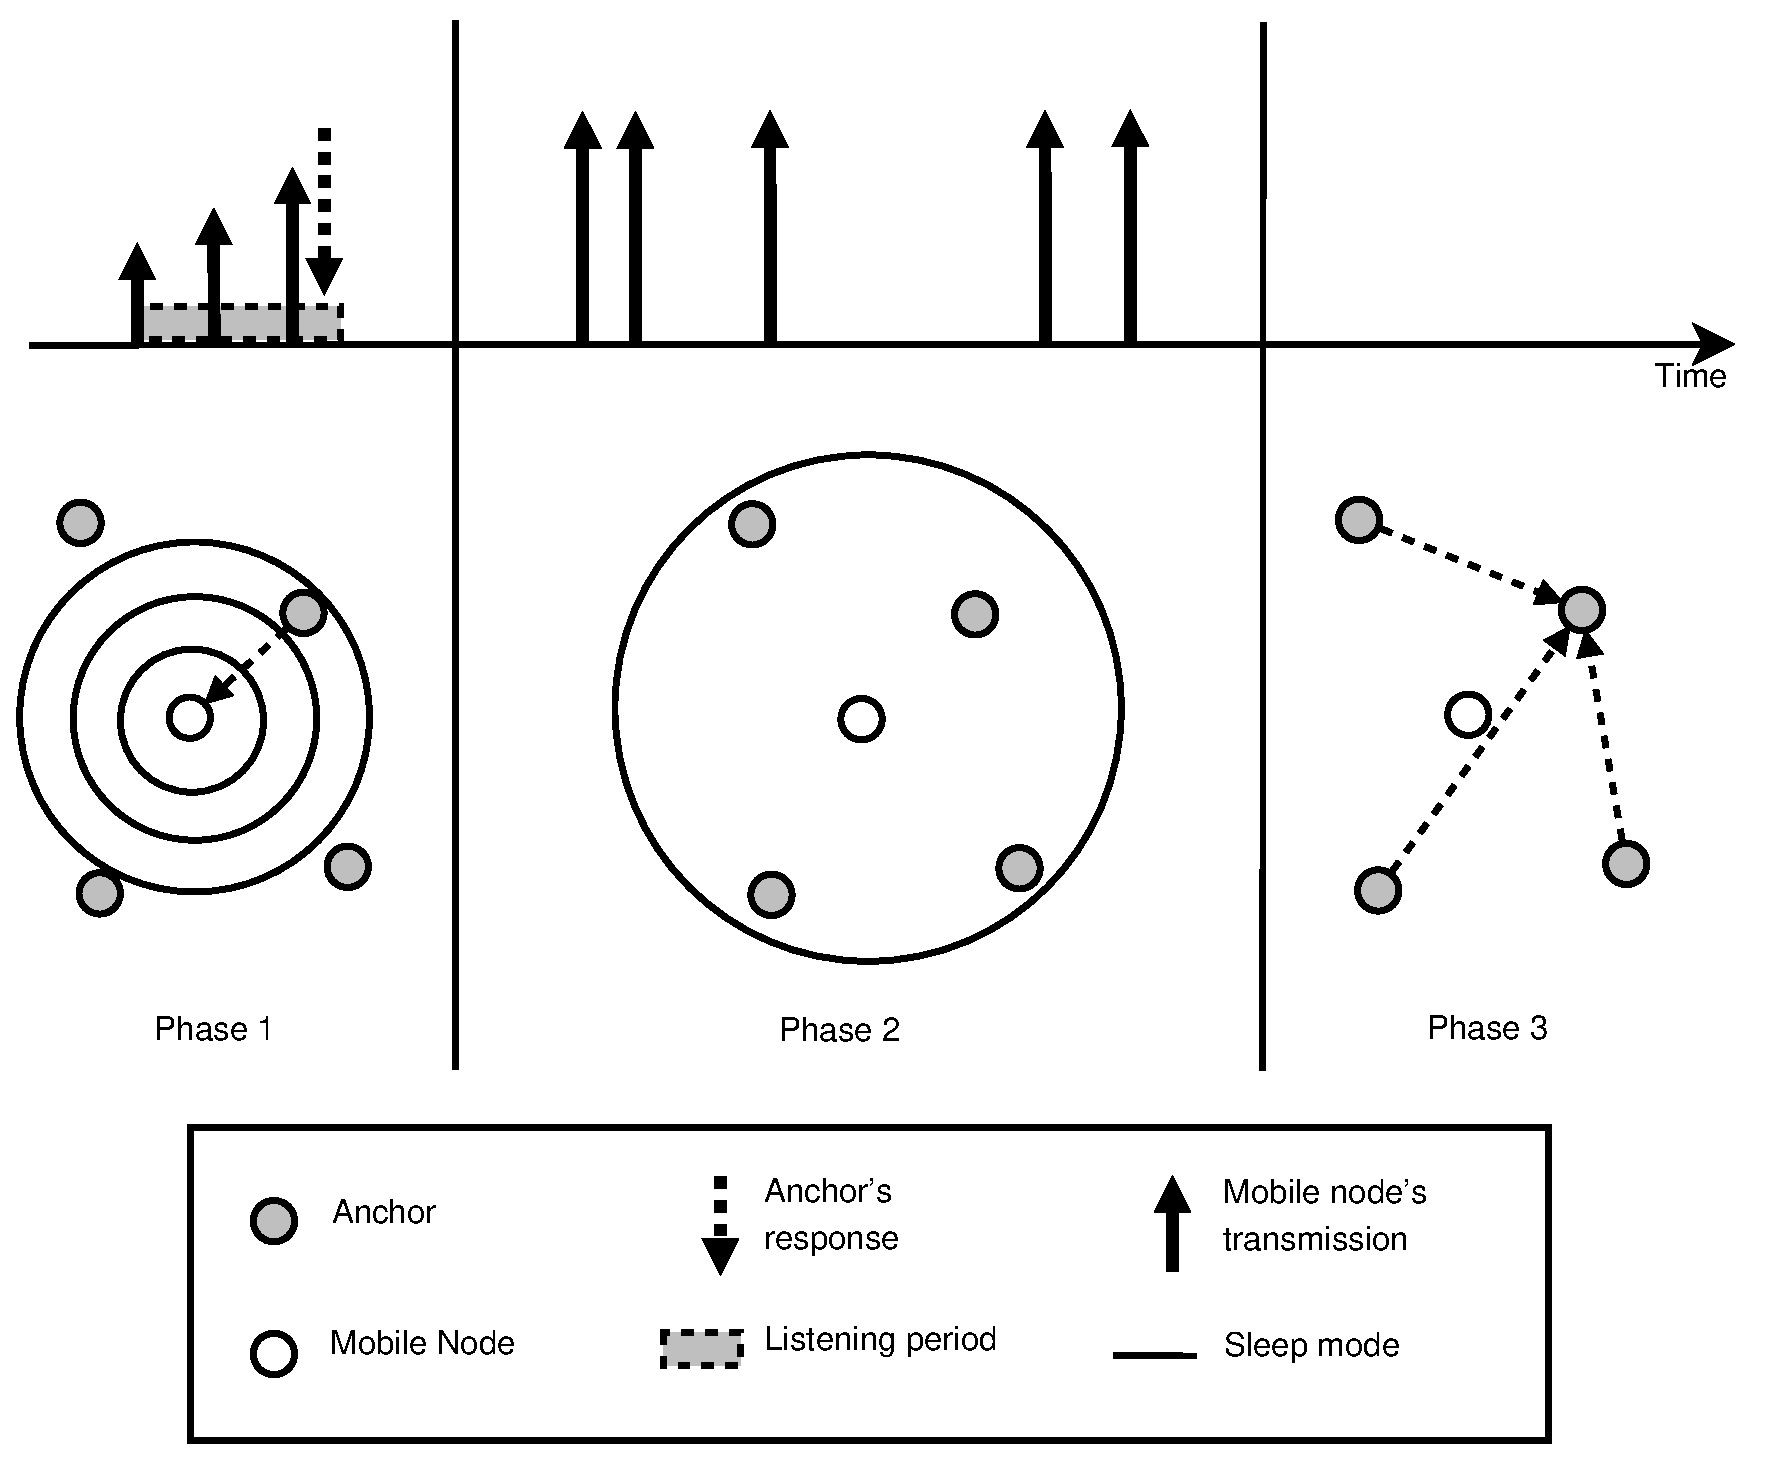
\includegraphics[width=0.7\textwidth]{LPL.eps}
 \end{center}
 \caption{LPL Phases \cite{LPLandOLP}}
 \label{fig:LPL}
\end{figure}

\begin{itemize}
 \item \textbf{Phase 1:} In this phase, \ac{MN} selects a random time to broadcast a synchronization request, starting with the minimum power,
and increasing this power until it receives an answer from an \ac{AN}, this will be the selected \ac{AN}, and the answer will contain information
about the phase times. This process makes sure that only the nearest \acp{AN} answer to this synchronization request. In the next phase 1, if 
the \ac{MN} needs to know its position, it asks its selected \ac{AN} about this information, and if not it just synchronizes.
 \item \textbf{Phase 2:} In phase 2, the \ac{MN} broadcasts several packets in random times to minimize the collisions. Any time the node is not
transmitting, it goes to sleep, this makes that \acp{MN} are awake only when they transmit eliminating this way the idle listening. The \acp{AN} that
received this broadcasts, store the read \ac{RSSI} values and the selected \ac{AN}.
 \item \textbf{Phase 3:} During this phase, the \acp{MN} sleeps and the \acp{AN} send the measured \ac{RSSI} values to the selected \ac{AN}. 
This \ac{AN} will calculate the \ac{MN} position in Distributed-A case or send the data to a central computer in Centralized case. In this phase is
also done the synchronization between \acp{AN} and network configuration.


\end{itemize}


\subsection{\acl{OLP}}

In the case of \ac{OLP} protocol and unlike \ac{LPL}, the \ac{MN} is the one who listens. This protocol is also divided in 3 phases, 2 of 
them can be appreciated in Figure \ref{fig:OLP}.

\begin{figure}[ht]
 \begin{center}
  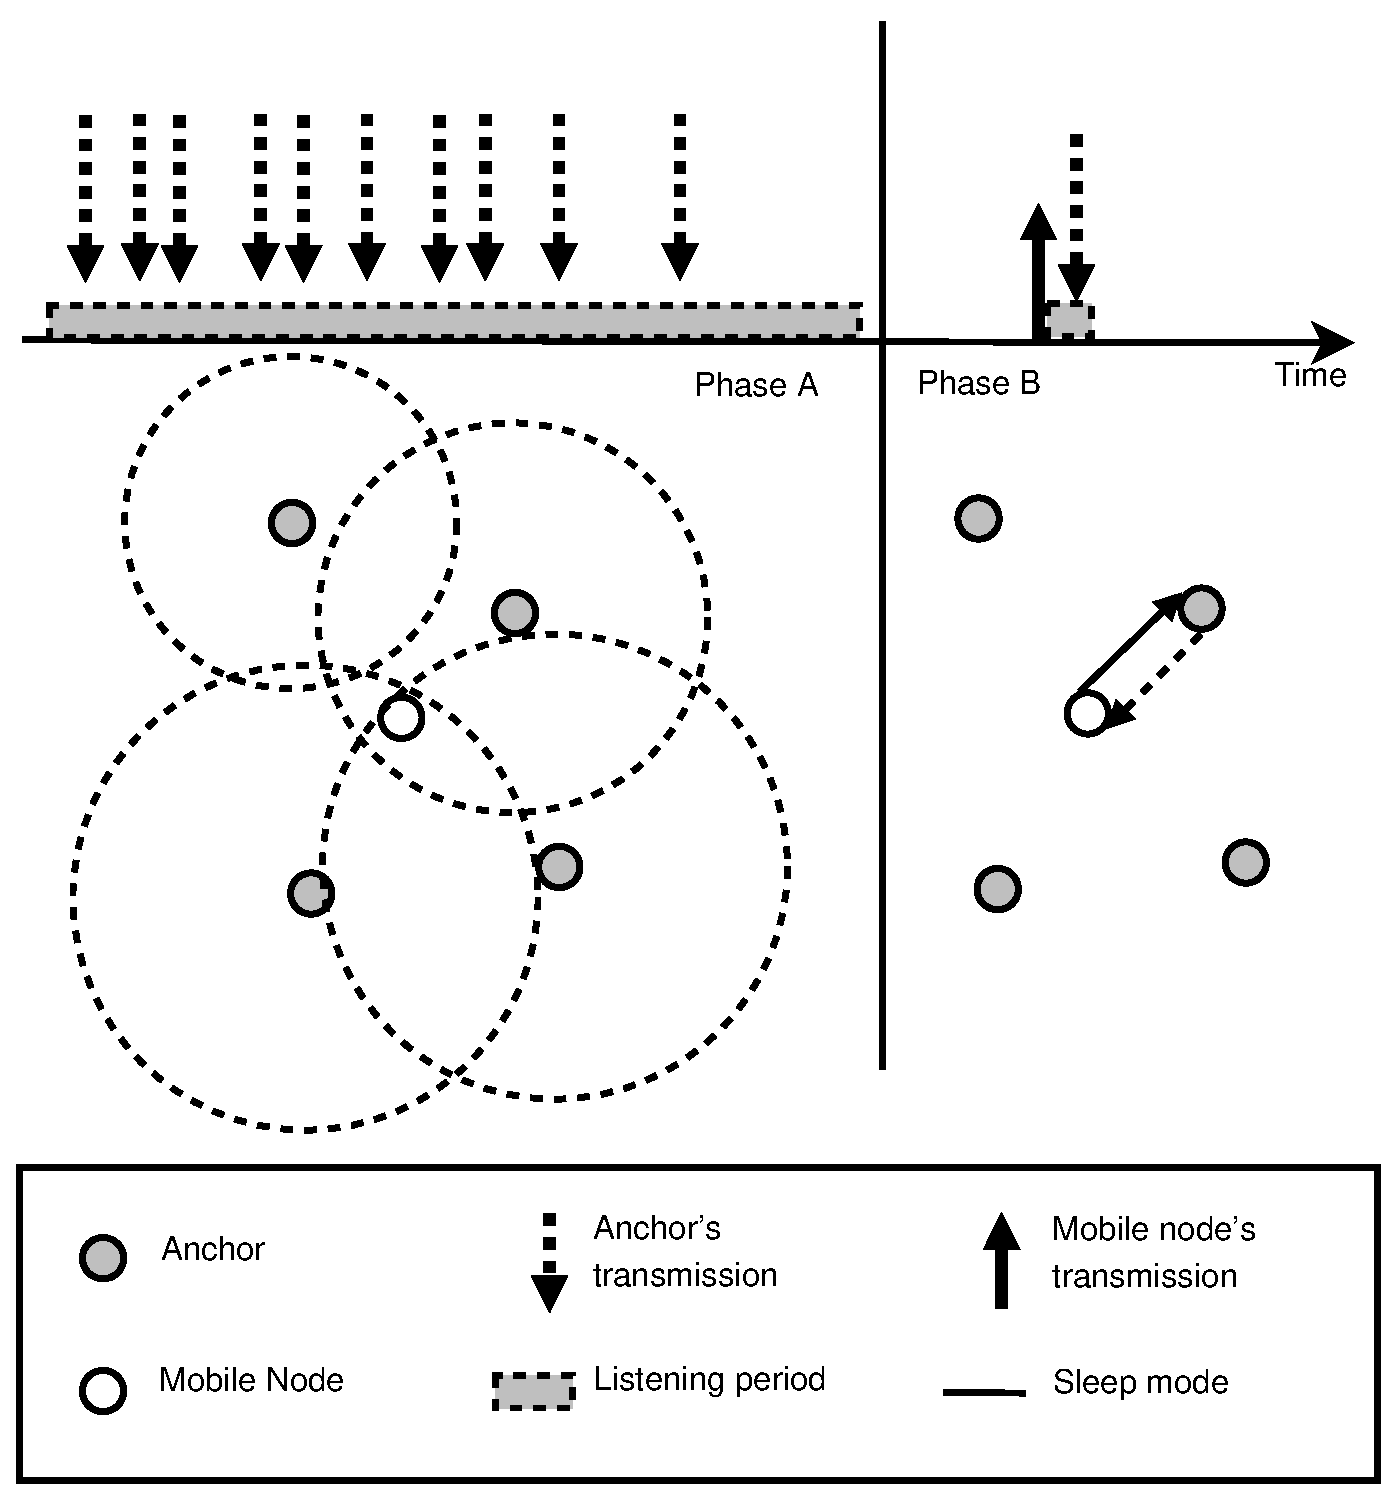
\includegraphics[width=0.5\textwidth]{OLP.eps}
 \end{center}
 \caption{OLP Phases \cite{LPLandOLP}}
 \label{fig:OLP}
\end{figure}

\begin{itemize}
 \item \textbf{Phase A:} In this phase, and thanks to the synchronization among \acp{AN}, the inter-arrival time is reduced, reducing so the
idle listening. This packets also content synchronization information for the \ac{MN}. In this phase \ac{RSSI} values are received and stored
by the \ac{MN}, and then it goes to sleep.
 \item \textbf{Phase B:} In this phase and in Distributed-M mode, the \ac{MN} will use easy localization algorithms together with all the \ac{RSSI}
values read to get its position. In case of Distributed-A or Centralized mode, the \ac{MN} will send a report to the selected \ac{AN}, took 
from the highest \ac{RSSI} value, with all the stored \ac{RSSI} values in Phase A. The selected \ac{AN} will answer with an \ac{ACK}. In next
phase B, the \ac{MN} will ask the selected \ac{AN} about its position in case it needs it.
 \item \textbf{Phase C:} Like in \ac{LPL} this Phase is reserved for communication among \acp{AN} and network configuration.
\end{itemize}


\section{High Configurable Protocol proposal}

From the previous section and according to the results in \cite{LPLandOLP}:
\begin{quote}
``LPL consumes lower energy than OLP when many RSSI samples are required from many ANs. On the other hand,
OLP becomes more energy efficient than LPL when there are several MNs and few RSSI samples are needed. \cite{LPLandOLP}''
\end{quote}

This makes clear the necessity of a Configurable Protocol able to vary the nodes behavior according to the current situation of the network
and the necessities of the node.

High correlation between RSSI values near in time.

Synchronization in the phases.

Centralized vs. Distributed.

Too much time listening to transmit, reduce cases with CSMA when battery is critic using broadcasts from nodes.

As it was seen, \ac{OLP} and \ac{LPL} protocols, are based in \ac{RSSI} values
This work is also based in localization using \ac{RSSI} values, although this work just proposes a framework for the protocol and does not try 
to locate any
node 
From the Table \ref{tab:wsn_applications} (page~\pageref{tab:wsn_applications}) where different applications for \ac{WSN} where stated, it is possible
to extract 4 different kind of nodes.

\section{Sync Phase detail}

\chapter{Protocol Implementation}
\label{chap:protocolimplementation}

\section{Used Tools}

\section{Sync Phase study development}

\ac{CSMA/CA} disabled to be able to calculate the time-stamp after the random time added in application layer.

\section{Framework development}

\chapter{Simulation and Results}
\label{chap:simulationandresults}

\section{Sync Phase simulation and analysis}

\section{Framework simulation and analysis}

\chapter{Conclusion and future work}
\label{chap:conclusionsandfuture}

Look for the best parameters in the simulation.

Change node configuration.

Move the nodes.

Comment how long the nodes would last with this protocol.

\bibliographystyle{plain}
\bibliography{bib}

\appendix
\chapter{Source code first contact}
\label{chap:installation}

\section{Git Introduction}

\section{OmNet++, \ac{MiXiM} and my code}


% Pages with extra content of the document
\appendix

\end{document}